%Template pembuatan proposal skripsi.
\documentclass{jtetiproposalskripsi}
\usepackage{url}

%-----------------------------------------------------------------
%Disini awal masukan untuk data proposal skripsi
%-----------------------------------------------------------------
\titleind{PERANCANGAN VoIP (VOICE OVER INTERNET PROTOCOL) MENGGUNAKAN ASTERISK}

\fullname{Alifan Alfun Salim}

\idnum{11 1065 1244}

\approvaldate{09 Januari 2015}

\degree{Sarjana Teknik Informatika}

\yearsubmit{2015}

\program{Teknik Informatika}

%\headprogram{Sarjiya, S.T., M.T., Ph.D.}
%\dept{Teknik Informatika}

\firstsupervisor{Triawan Adi Cahyanto}
\firstnip{}

\secondsupervisor{Eko Fajar Yanuwarsa}
\secondnip{}


%-----------------------------------------------------------------
%Disini akhir masukan untuk data proposal skripsi
%-----------------------------------------------------------------

\begin{document}

\cover

\approvalpage

%-----------------------------------------------------------------
%Disini akhir masukan untuk muka skripsi
%-----------------------------------------------------------------

%-----------------------------------------------------------------
%Disini awal masukan Intisari
%-----------------------------------------------------------------
\begin{abstractind}
\emph{Voice over Internet Protocol} (VoIP) adalah komunikasi suara melalui jaringan IP. Pada penelitian ini dirancang sistem IP PBX dengan menggunakan teknologi berbasis \emph{VoIP}. IP PBX adalah perangkat \emph{switching} komunikasi telepon dan data berbasis teknologi \emph{Internet Protocol} (IP) yang mengendalikan ekstension telepon analog maupun \emph{ekstension IP Phone}. 

Software VirtualBox digunakan dengan tujuan agar lebih memudahkan dalam sistem pengoperasian Linux yang dimana program untuk membuat IP PBX adalah menggunakan Briker yang bekerja pada Operating System CentOS 5.1 dan aplikasi Asterisk. Setelah proses penginstalan pada Virtualbox dilakukan implementasi jaringan IP PBX. Setelah mengimplementasikan jaringan IP PBX sesuai dengan topologi, kemudian melakukan pengujian success call rate dan analisis \emph{Quality of Service} (QoS). Pengukuran QoS menggunakan parameter jitter, delay, dan packet loss yang dihasilkan dalam sistem IP PBX ini. Sedangkan nilai pacet loss yang didapat pada saat user 1 sebagai pemanggil telepon kadala 0\%. Sedangkan persentase packet loss pada saat user 1 sebagai penerima telepon adalah 0,01\%. Nilai delay pada saat berkomunikasi antar user berada pada 11,75 ms.

Secara keseluruhan nilai yang didapatkan melalui penelitian ini, dimana hasil pengujian parameter-parameter QOS sesuai dengan standar yang telah direkomendasikan oleh itu dan didapatkan nilai QoS dengan hasil “baik”.


\bigskip
\textbf{Kata kunci} : \emph{VirtualBox}\emph{CentOS 5.1}, \emph{Asterisk}, \emph{X-Lite Soft phone}.
\end{abstractind}
%-----------------------------------------------------------------
%Disini akhir masukan Intisari
%-----------------------------------------------------------------

\tableofcontents
\addcontentsline{toc}{chapter}{DAFTAR ISI}
\selectlanguage{bahasa}\clearpage\pagenumbering{arabic}\setcounter{page}{1}

%-----------------------------------------------------------------
%Disini awal masukan untuk Bab
%-----------------------------------------------------------------
\chapter{LATAR BELAKANG}

\section{Latar Belakang Masalah}
Teknologi jaringan komputer dan internet saat ini telah  menjadi salah satu kebutuhan yang penting dalam aktifitas kehidupan. Setiap hari terus  berkembang, perkembangan yang ramai dibicarakan dan dibahas sekarang ini adalah teknologi yang mengarah pada \emph{Next  Generation Network} (NGN) yang kemungkinan besar akan berplatform pada teknologi \emph{Internet Protocol} (IP), salah satu teknologi yang mulai digunakan adalah softswitch  atau yang dikenal dengan nama \emph{Voice over Internet Protocol} (VoIP). 

Dengan adanya teknologi VoIP, merupakan kabar baik bagi pengguna telepon, karena setiap orang  dapat berkomunikasi tanpa harus menggunakan pulsa telepon dalam jaringan VoIP. Di Indonesia,  salah satu  penggerak  pertama  telepon  internet  adalah  \emph{VoIP}  Merdeka  yang dipimpin  oleh  Bapak Onno W. Purbo. Setelah itu muncul \emph{VoIP} Rakyat (http://www.voiprakyat.or.id) yang merupakan komunitas riset  dan pengembangan teknologi VoIP berbasis open sourceyang dikembangkan di bawah kepemimpinan Bapak Anton Raharja dengan timnya.

\emph{VoIP} dapat  diimplementasikan pada suatu perusahaan, kantor, kampus, atau perumahan, baik melalui sambungan internet atau melalui jaringan lokal. Pada dasarnya syarat utama  yang  harus dipenuhi dalam \emph{VoIP}, yaitu (1) mempunyai  sambungan  ke internet, dan atau  (2) mempunyai \emph{provider VoIP} atau operator telekomunikasi secara langsung. Pilihan pertama menggunakan  internet  publik  biasanya  dilakukan  jika menginginkan  untuk  mengakses  internet sekaligus dengan VoIP, sementara pilihan kedua dilakukan jika ingin melakukan banyak hubungan komunikasi \emph{VoIP} dengan operator telekomunikasi di Indonesia.

\emph{VoIP} juga dapat dibangun dalam jaringan lokal yang dapat menghubungkan antar divisi.  Biasanya suatu kantor atau kampus sudah memiliki komputer pada tiap divisi bahkan pada tiap ruang kerja, kondisi ini dapat dimanfaatkan untuk mempermudah komunikasi antar divisi. Penggunaan komputer di sini menjadi hal yang sangat penting, karena \emph{VoIP} yang akan dibangun  membutuhkan komputer, hand phone, dan sound card.

Teknologi \emph{VoIP} secara umum terdapat 2 protokol, yaitu H.323 dan \emph{Session Initiation Protocol} (SIP). Namun saat ini, protokol \emph{SIP} yang lebih banyak  dipakai  karena  lebih  mudah  cara  pemakaiannya.  Software yang digunakan  untuk  server dan  client VoIP  dapat  diambil  secara  gratis  dan open source di internet. Penggunaan peralatan  yang  berbasis SIP semakin hari semakin banyak dan harga peralatannya juga semakin murah. Softswitch yang biasa digunakan menggunakan software asterisk yang dapat diambil dari (http://www.asterisk.org).  Softswitch adalah  sentral  telepon  yang  dapat dioperasikan  di  komputer biasa atau disebut server VoIP. Sementara telepon  yang paling sederhana  berupa  softphone di Personal Computer (PC) seperti x-lite dan SJ Phone yang bisa diambil gratis di internet.

Untuk membuat sentral telepon \emph{VoIP}, yang perlu dilakukan adalah instalasi \emph{softswitch} seperti \emph{asterisk} di komputer server serta instalasi \emph{softphone} di komputer client. Perlu diperhatikan, informasi yang  dibutuhkan  agar  interkoneksi  dapat  dilakukan  adalah  username, password dan  server atau softswitch dimasukkan  ke  konfigurasi  softswitch asterisk,  maka  setiap  client dapat  dengan  mudah  me-register  softswitch yang digunakan pada sentral telepon. Dengan tersambungnya softswitch ke sentral  telepon,  maka  pembicaraan atau call VoIP  dapat  dilakukan  dari area yang berbeda ke jaringan \emph{VoIP}.
	
Dari keterangan di atas, maka penulis berkeinginan untuk membangun dua sentral telepon \emph{VoIP}  dalam jaringan lokal dan menggunakan \emph{softphone} untuk komunikasi clientnya.


\section{Rumusan Masalah}
Dalam pembuatan sebuah sistem , tentu tidak akan terlepas dari beberapa permasalahan. Dari latar belakang permasalahan diatas maka, dapat disimpulkan permasalahan yang ada yaitu sebagai berikut:

\begin{enumerate}
\item Bagaimana mengimplementasikan layanan \emph{VoIP} dalam jaringan \emph{LAN} yang berbasis \emph{protocol SIP} ?
\item Bagaimana melakukan manajemen \emph{QoS} untuk layanan VoIP pada jaringan LAN, di mana di dalamnya juga terdapat layanan data lainnya?
\item Bagaimana mengintegrasikan \emph{VoIP} ke \emph{PABX} ?
\item Bagaimana mengoperasikan \emph{Asterisk}?
\end{enumerate}

\section{Batasan Masalah}
Karena pembahasan masalah \emph{VoIP} meliputi aspek yang cukup luas, penulis hanya membahas mengenai perancangan sentral telepon VoIP dalam jaringan internet antar ruangan menggunakan Personal Computer (PC) dan softwarephone \emph{(sofphone)} untuk berkomunikasi clientnya, dan penelitian ini akan dibatasi pada permasalahan berikut :

\begin{enumerate}
\item Parameter yang digunakan untuk mengamati kualitas layanan meliputi bandwith, jitter, MOS, dan packet loss.
\item Diasumsikan kondisi kanal sempurna, yaitu tidak ada trsnmission error dan link adaptions.
\item Pengalamatan IP mengggunakan IP versi 4.
\item Menggunakan asterisk 32 sebagai \emph{server VoIP}
\end{enumerate}

\section{Tujuan Penelitian}
Berdasarkan permasalahan yang diteliti, maka maksud dari penulis tugas akhir ini adalah untuk mendesain dan menganalisa jaringan komunikasi \emph{VoIP} Perbasi protokol SIP.
Sedangkan tujuan yang akan dicapai dalam penelitian ini adalah :
\begin{enumerate}
\item jaringan telepon berbasis IP menggunakan layanan \emph{VoIP}.
\item Mengetahui parameter-parameter yang diperlukan agar jaringan VoIP yang dibangun dapat berjalan secara optimal.
\item Mengetahui bagaimana perubahan performasi dari \emph{VoIP} sebelum dan sesudah diterapkan \emph{Qos} dengan menganalisa \emph{jitter}, \emph{packet loss} dan \emph{MOS}
\end{enumerate}

\section{Manfaat Penelitian}
Manfaat dari penelitian ini adalah memanfaatkan jaringan \emph{fiber optik} (FO) di lingkungan Universitas Muhammadiyah Jember untuk menekan biaya operasional dalam melakukan komunikasi suara atau video melalui jaringan IP secara local/intranet dan memudahkan berkomunikasi di jaringan lokal.

%-------------------------------------------------------------------------------
\chapter{TINJAUAN PUSTAKA DAN DASAR TEORI}                

\section{Tinjauan Pustaka}
Pada bagian ini berisi referensi yang relevan. Tinjauan pustaka ini menguraikan teori, temuan dan bahan perancangan pembangunan untuk menyusun kerangka pemikiran atau konsep yang akan digunakan dalam perancangan.

\begin{figure}[!htbp]
\centering
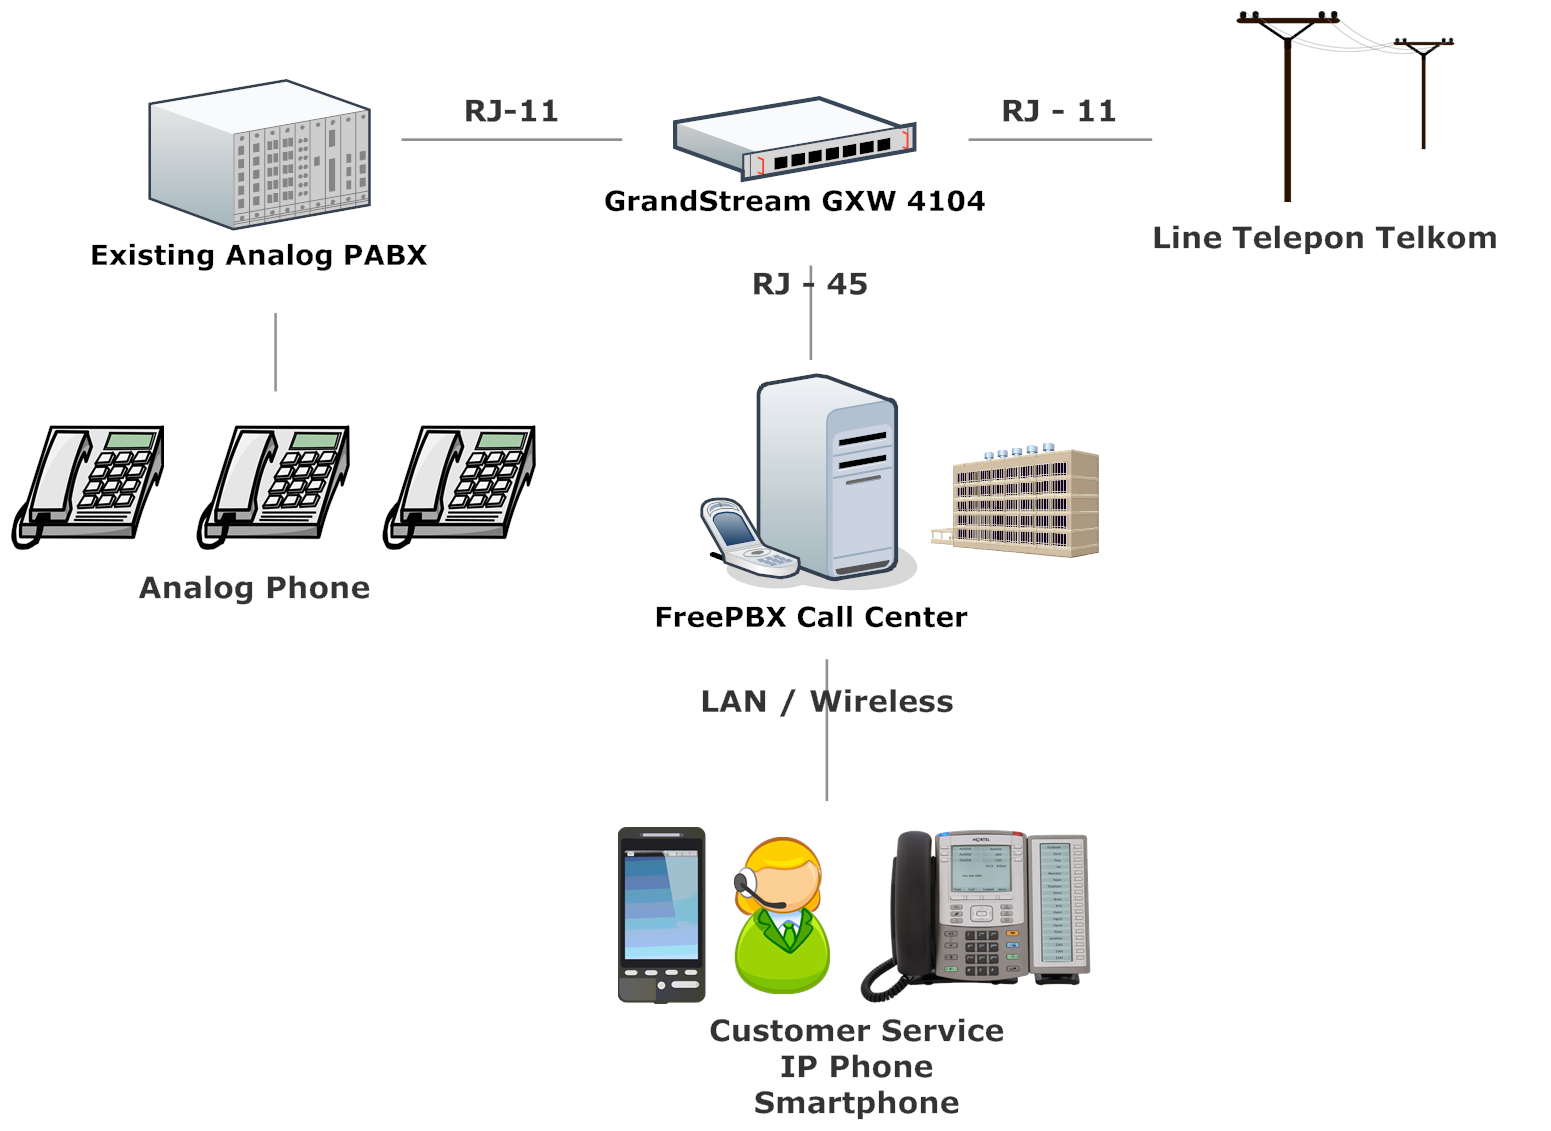
\includegraphics[width=10cm,height=10cm]{gambar/voip-gateway}
\caption{voip-gateway}
\label{penanda}
\end{figure}

Seperti yang sudah disebutkan sebelumnya, untuk dapat terhubung informasi yang dibutuhkan  agar interkoneksi dapat dilakukan adalah username, password dan  server/softwitch dimasukkan ke konfigurasi softswitch asterisk, maka setiap client dapat dengan mudah me-register softswitch yang digunakan pada sentral telepon. Dengan tersambungnya softswitch ke sentral telepon, maka pembicaraan atau \emph{call VoIP} dapat dilakukan dari area yang berbeda ke jaringan \emph{VoIP}.

\section{VOIP (Voice Over Internet Protocol)}
%\subsection{\emph{Wireless Sensor Network}}%
Voice over internet protokol juga disebut VoIP, IP Telephony, Internet Telephony atau (Digital Phone) adalah teknologi yang memungkinkan percakanpan suara jarak jauh melalui media internet. Data suara diubah menjadi kode digital dan dialirkan melalui jaringan yang mengirimkan paket-paket data, dan bukan lewat sirkuit analog telephone biasa secara real time.

\section{Lan (Local Area Network)}
\emph{Lan (Local Area Network)} adalah jaringan komputer yang jaringannya mencakup wilayah kecil; seperti jaringan komputer kampus, degung-gedung, kantor, dalam rumah, sekolah atau yang lebih kecil. Saat ini kebanyakan  lan berbasis pada teknologi IEEE 802.3 Ethernet menggunakan pernagkat switch, yang mempunyai transfer data 10, 100, atau 1000 Mbit/s.

\section{Qos (Quality Of Service)}
\emph{Qos} (Quality of Service) adalah kemampuan untuk memberikan prioritas yang berbeda untuk berbagai aplikasi, pengguna, atau aliran data, atau untuk menjamin tingkat tertentu kinerja ke aliran data. Misalnya, diperlukan sedikit menilai, keterlambatan, naik opelet, probabilitas dropping paket dan / sedikit kesalahan menilai mungkin dilakukan. Menjamin kualitas layanan merupakan hal penting jika kapasitas jaringan yang memadai, terutama untuk aplikasi real-time streaming multimedia seperti VoIP, game online dan IP-TV, karena ini sering memerlukan kecepatan tetap dan peka terhadap penundaan (delay), dan dalam jaringan di mana kapasitas adalah sumber daya terbatas, misalnya dalam komunikasi data selular. Pada jaringan yang tidak terdapat kongesti/tabrakan, mekanisme QoS yang tidak diperlukan.

\section{Asterisk}
\emph{Asterisk} adalah software IP IPX untuk membuat sistem layanan komunikasi telepon melalui internet atau biasa disebut \emph{VoIP} (Voice over Internet Protocol). Asterisk adalah software Open Source yang berjalan di Linux. Asterisk juga memungkinkan komunikasi antar pengguna telepon regular dengan telepon berbasis sip (sip phones).

%-------------------------------------------------------------------------------
\chapter{METODOLOGI}
\section{Metodelogi Penelitian}
Merupakan bentuk kegiatan identifikasi terhadap perancangan yang dilakukan.
Pada tahap ini penulis mengelompokkan ke dalam 3 metode yaitu :
\begin{enumerate}
\item Metode Observasi (penelitian).
\newline Metode yang dilakukan dengan cara melakukan pengamatan secara sistematis aktif dan mencatat hal-hal yang diperlukan dalam pembuatan desain dan pengolahan data proses.
\item Metode Studi Pustaka 
\newline Pengumpulan data dengan cara mengumpulkan literatur, jurnal, paper, dan bacaan-bacaan yang akan dibahas dengan bersumber buku-buku yang ada kaitannya dengan judul penelitian untuk membantu menyelesaikan pembangunan dalam sistem ini.
\item Metode Pendataan 
\newline Metode untuk mengarsip berkas-berkas yang terkait dengan objek penelitian meliputi berkas pendataan dan laporan hasil.
\item Desain Sistem 
\newline Perancangan VoIP Server menggunakan Asterisk dengan sistem operasi Linux. Pada bagian ini akan dilakukan proses desain VoIP server dan juga menggambarkan topologi yang akan digunakan.
\end{enumerate}
\section{Alat dan Bahan}
Asterisk adalah implementasi perangkat lunak dari “telephone private branch exchange (PBX)”, diciptakan pada tahun 1999 oleh Mark Spencer dari Digium. Seperti PBX lainnya, dimungkinkan memasang pesawat telepon dan melakukan panggilan ke satu dengan lainnya, termasuk tersambung ke layanan telepon pribadi dan publik, termasuk layanan jaringan telepon umum (PSTN) dan Voice over Internet Protocol (VoIP). Nama Asterisk berasal dari * (tanda bintang). Asterisk dirilis menganut model lisensi ganda, menggunakan GNU/GPL sebagai lisensi perangkat lunak bebas dan lisensi perangkat lunak berpemilik untuk mengizinkan pemegang lisensi untuk mendistribusikan komponen sistem proprietari yang tidak perlu dipublikasikan.

\section{Analisa dan Kesimpulan}
Setelah dilakukan pengujian terhadap semua sistem, tahapan terakhir adalah menganalisa paket data yang dibutuhkan ketika program berjalan melakukan panggilan baik menggunakan PABX ataupun softphone (X-LITE). Setelah itu dibuat kesimpulan sesuai dengan hasil analisanya

\section{Jadwal Kegiatan}
Penelitian direncanakan akan dilaksanakan selama enam bulan. Rincian rencana jadwal penelitian dicantumkan dalam tabel berikut.

\begin{center}
Tabel 3.1. Jadwal Penelitian.
\end{center}
\vspace{-0.5cm}
\begin{figure}[ht!]
  \centering
    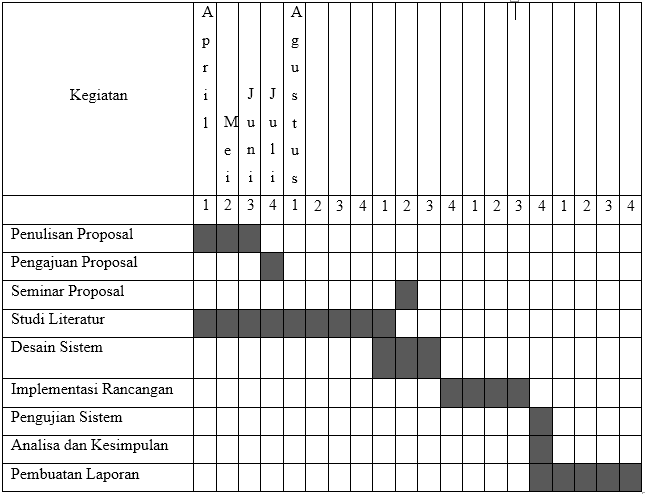
\includegraphics[width=13cm]{gambar/jadwal}
\end{figure}

%-----------------------------------------------------------------
%Disini akhir masukan Bab
%-----------------------------------------------------------------

%-----------------------------------------------------------------
%Disini awal masukan untuk Daftar Pustaka
%-----------------------------------------------------------------
%%\nocite{Abel2010,Guerbas201350}
%%\bibliography{research-plan}
%%\bibliographystyle{plainnat}
\begin{thebibliography}{9}

\bibitem[satu(2013)]{satu01}
Nurkholis, A., \& Hendrawan, A. (2011). Implementasi Server VoIP untuk Komunikasi di PT. Lintas Data Prima. Yogyakarta: STMIK AMIKOM

\bibitem[dua(2013)]{dua02}
Putra, A. Y. (2010). Analisis Dan Perancangan Security Voice Over Internet Protokol ( VoIP ) Menggunakan GNU LINUX TRIBOX pada Jaringan Lokal. Yogyakarta: STMIK AMIKOM.

\bibitem[tiga(2013)]{tiga03}
Dokument online, \url{http://gudanglinux.com/glossary/asterisk/}, diakses pada  Januari 2015

\bibitem[empat(2013)]{empat04}
Dokumen online, \url{http://id.wikipedia.org/wiki/Voice_over_IP}, diakses pada  Desember 2014

\bibitem[lima(2013)]{lima05}
Dokument online, \url{http://id.wikipedia.org/wiki/Jaringan_wilayah_lokal}, diakses pada  Desember 2014

\bibitem[enam(2013)]{enam06}
Dokumen online, \url{http://opensource.telkomspeedy.com/wiki/index.php/QoS/}, diakses pada Desember 2014


\end{thebibliography}
\addcontentsline{toc}{chapter}{DAFTAR PUSTAKA}
%-----------------------------------------------------------------
%Disini akhir masukan Daftar Pustaka
%-----------------------------------------------------------------

\end{document}
